\documentclass[11pt]{article}
\usepackage[margin=1.1in]{geometry}
\usepackage{amsmath,amssymb}
\usepackage{graphicx}
\usepackage{booktabs}
\usepackage{float}
\usepackage[hidelinks]{hyperref}

% Self-contained for Overleaf: all assets live inside this project folder.
% Place figure files in ./figures/ (no parent-relative paths).
\graphicspath{{figures/}}

\newcommand{\dd}{\mathrm{d}}
\newcommand{\Pmod}{P_{\mathrm{mod}}}

% TODO: title / authors / date
\title{}
\author{}
\date{}

\begin{document}
\maketitle

\begin{abstract}
% TODO: abstract
\end{abstract}

\section{Background}
\label{sec:background}

\section{Methods}
\label{sec:methods}

\subsection{Sequential per-segment Newton controller}
\label{sec:methods:controller}

The scan path is divided into control blocks that are optimized in execution
order. The control vector for block $i$ is given in Equation~\eqref{eqn:control_vector}.
\begin{equation}
	\label{eqn:control_vector}
  \mathbf{u}_i = (\Pmod{}_{,i},\,\sigma_i,\,v_i)^{\mathsf T},
  \qquad P_i=P_0\Pmod{}_{,i},
\end{equation}
Here, $\Pmod{}_{,i}$ is the absorbed-power multiplier, $\sigma_i$ is the lateral
beam standard deviation, and $v_i$ is the scan velocity. The melt-pool
half-width $w_i$ (the transverse semi-span from the scan centreline to the
liquidus boundary) and depth $d_i$ for a given set of control parameters
$\mathbf{u}_i$ are evaluated at the end of the block and compared
with the developed single-track targets $(w^*,d^*)$ through the normalized
residual given in Equation~\eqref{eq:normalized-residual}.
\begin{equation}
  \widetilde{\mathbf r}_i(\mathbf u_i)=
  \begin{pmatrix}
    (w_i-w^*)/w^*\\
    (d_i-d^*)/d^*
  \end{pmatrix}.
  \label{eq:normalized-residual}
\end{equation}
Figure~\ref{fig:controller-block} summarizes this causal block update: a
change made at $x_i$ is judged by how closely the melt-pool dimensions at
$x_{i+1}$ approach their targets.

\begin{figure}[H]
\centering
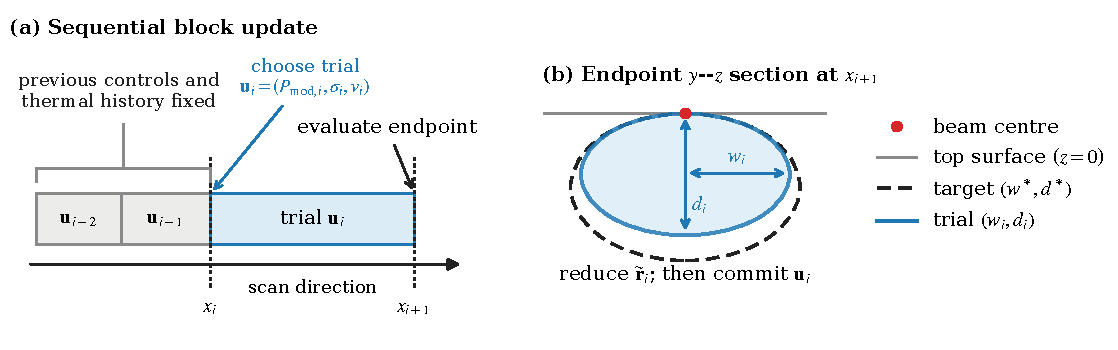
\includegraphics[width=0.96\textwidth]{controller_block_schematic.pdf}
\caption{Sequential control-block update. Previously accepted controls define
the fixed thermal history up to $x_i$. A trial control $\mathbf u_i$ is
applied over $[x_i,x_{i+1}]$, and its endpoint width and depth are compared
with the single-track targets in a transverse $y$--$z$ melt-pool section. }
\label{fig:controller-block}
\end{figure}

The controls
already accepted for blocks $j<i$ are replayed as fixed thermal history, so
the update for block $i$ cannot alter any preceding portion of the scan.
The approach is therefore a greedy optimization: the controls at block $i$ are
chosen to give the best possible melt-pool dimensions at its endpoint
$x_{i+1}$, then frozen before block $i{+}1$ is optimized. Since each block
looks only one block ahead and never revisits an earlier decision, the
schedule is optimal block-by-block but not necessarily globally.

The temperature field and its derivatives with respect to the current
block's power, beam width, and velocity are evaluated in one simulation using
first-order order-truncated imaginary (OTI) arithmetic. Spatial temperature
gradients and control derivatives on the liquidus isotherm are converted to
derivatives of $w_i$ and $d_i$ using the implicit function theorem. This gives
the Jacobian in Equation~\eqref{eq:control-jacobian}.
\begin{equation}
  J_i =
  \begin{pmatrix}
    \partial w_i/\partial\Pmod{}_{,i} &
    \partial w_i/\partial\sigma_i &
    \partial w_i/\partial v_i\\
    \partial d_i/\partial\Pmod{}_{,i} &
    \partial d_i/\partial\sigma_i &
    \partial d_i/\partial v_i
  \end{pmatrix}.
  \label{eq:control-jacobian}
\end{equation}
Residuals and controls are scaled, with
$S=\operatorname{diag}(1,200~\mu\mathrm{m},3~\mathrm{m\,s^{-1}})$ collecting the
nominal magnitude of each control (Table~\ref{tab:study-parameters}), so that
the scaled step $\Delta\mathbf z$ is dimensionless and a single $\lambda$
regularizes the three controls evenly. A Levenberg--Marquardt (regularized
Gauss--Newton) step is then computed as in Equation~\eqref{eq:regularized-newton}.
\begin{equation}
  (\widetilde J_i^{\mathsf T}\widetilde J_i+\lambda I)\Delta\mathbf z
  =-\widetilde J_i^{\mathsf T}\widetilde{\mathbf r}_i,
  \qquad
  \Delta\mathbf u_i=S\Delta\mathbf z,
  \label{eq:regularized-newton}
\end{equation}
where $\lambda=2.5\times10^{-2}$ and $\widetilde J_i$ is the target-normalized
Jacobian in scaled control coordinates,
so that $\widetilde J_i\,\Delta\mathbf z$ is precisely the first-order change in
the normalized residual $\widetilde{\mathbf r}_i$ produced by the scaled step
$\Delta\mathbf z$. Since the update is underdetermined, the width--depth
residual alone does not determine a unique step: a family of $(\Pmod,\sigma,v)$
corrections can produce the same first-order geometric change. Thus, a small penalty is
 placed on departures from the nominal velocity, which resolves this
degeneracy by preferring the correction closest to nominal speed, without
allowing a worse geometric residual to be accepted.

The update is safeguarded by componentwise per-iteration step-size caps of
$0.5$ in $\Pmod$, $80~\mu$m in $\sigma$, and $1.5$~m\,s$^{-1}$ in $v$, together
with the bounds
\begin{equation}
  0.05\leq\Pmod\leq3,
  \qquad 80\leq\sigma\leq400~\mu\mathrm{m},
  \qquad 0.5\leq v\leq8~\mathrm{m\,s^{-1}}.
\end{equation}
Because the step is derived from a linearized model, its full length can step
beyond the region where the linearization is accurate, so the predicted
reduction in the residual is not realized. A trial control
$\mathbf u_i+\alpha\,\Delta\mathbf u_i$ is therefore formed with a backtracking
step-length factor $\alpha\in\{1,1/2,1/4,1/8,1/16\}$, and the first value that
decreases the physical merit
$\tfrac12\lVert\widetilde{\mathbf r}_i\rVert_2^2$ is accepted; if none does, no
update is taken. A block is
accepted without an OTI evaluation if a preliminary double-precision replay
is already within a $5\%$ endpoint tolerance; otherwise, at most six Newton
iterations are taken.

The first block after each turnaround is initialized with a deliberately cool,
slow guess ($P=30$~W, $\sigma=200~\mu$m, and $v=1$~m\,s$^{-1}$). Because the
material just past a turnaround is still hot from the adjacent track,
warm-starting this block from the preceding high-speed controls would pin the
Newton iteration in a spurious high-velocity local solution; the cool, slow
guess avoids that basin. Each later block on the same track is instead
warm-started from the immediately preceding optimized block, promoting smooth
control transitions along the scan. The accepted controls are then committed to
the scan history before the next block is optimized.

\section{Results}
\label{sec:results}

The studies below use the common material and nominal process conditions in
Table~\ref{tab:study-parameters}. These conditions match those used by
Stump and Plotkowski~\cite{stump2019}. Parameters are varied only where stated.
Melt-pool widths are reported here as the full transverse span, i.e.\ twice the
half-width $w_i$ regulated by the controller; the normalized residual and
Jacobian make this a matter of convention only.

\begin{table}[H]
\centering
\small
\begin{tabular}{@{}lll@{}}
\toprule
parameter & symbol & value\\
\midrule
\multicolumn{3}{@{}l}{\textit{Material and thermal properties}}\\
thermal conductivity & $k$ & 26.6 W\,m$^{-1}$K$^{-1}$\\
specific heat capacity & $c_p$ & 600 J\,kg$^{-1}$K$^{-1}$\\
density & $\rho$ & 7451 kg\,m$^{-3}$\\
initial temperature & $T_0$ & 1273 K\\
liquidus temperature & $T_{\mathrm{liq}}$ & 1610 K\\
\addlinespace
\multicolumn{3}{@{}l}{\textit{Nominal process conditions}}\\
absorbed beam power & $P_0$ & 150 W\\
lateral beam standard deviation & $\sigma_{xy,0}$ & 200 $\mu$m\\
absorption-depth standard deviation & $\sigma_z$ & 10 $\mu$m\\
scan speed & $v_0$ & 3 m\,s$^{-1}$\\
hatch spacing & $h$ & 0.1 mm\\
tracking timestep & $\Delta t$ & 50 $\mu$s\\
\bottomrule
\end{tabular}
\caption{Material properties and nominal process conditions used throughout
the two-track, square, and triangle studies.}
\label{tab:study-parameters}
\end{table}

\subsection{Two-track base case}
\label{sec:results:twotrack}

The two-track case is the smallest geometry considered that contains both a
single turnaround and thermal interaction between neighbouring tracks. It
therefore provides a compact base case for evaluating the optimization
procedure, isolating turnaround behaviour, and selecting an appropriate
control-block length before moving to full raster geometries. The simplest
control policy is considered: continuous serpentine scanning in which only the
power $P$, lateral beam width $\sigma$, and scan velocity $v$ are modulated,
compared against the unoptimized nominal serpentine. Each scan line is
divided into uniform control blocks, and the block length is varied from $5$
to $0.1$~mm. This sweep identifies $1$~mm as a suitable working block length
for the larger square and triangle studies, as demonstrated in
Table~\ref{tab:twotrack-block}.

\begin{table}[H]
\centering
\small
\begin{tabular}{lc}
\toprule
control block & tracked depth ($\mu$m)\\
\midrule
unoptimized baseline & $69.4 \pm 12.4$\\
$5$~mm    & $65.1 \pm 9.4$\\
$2.5$~mm  & $63.4 \pm 7.8$\\
$1$~mm    & $\mathbf{62.5 \pm 6.6}$\\
$0.5$~mm  & $68.4 \pm 10.3$\\
$0.1$~mm  & $101.6 \pm 16.3$\\
\bottomrule
\end{tabular}
\caption{Two-track block-length sweep for the continuous $P/\sigma/v$ policy:
beam-on tracked melt-pool depth (mean~$\pm$~standard deviation) about the
developed single-track target. Regulation is tightest at $1$~mm; the tested
$0.5$ and $0.1$~mm schedules destabilize.}
\label{tab:twotrack-block}
\end{table}

The spatial outcome, optimized control history, and transient response of the
selected $1$~mm controller are shown in
Figures~\ref{fig:twotrack-maps}--\ref{fig:twotrack-traces}. Relative to the
nominal serpentine, the tracked depth standard deviation falls from $12.4$ to
$6.6~\mu$m and the surface fusion-depth standard deviation from $9.2$ to
$4.4~\mu$m.

\begin{figure}[H]
\centering
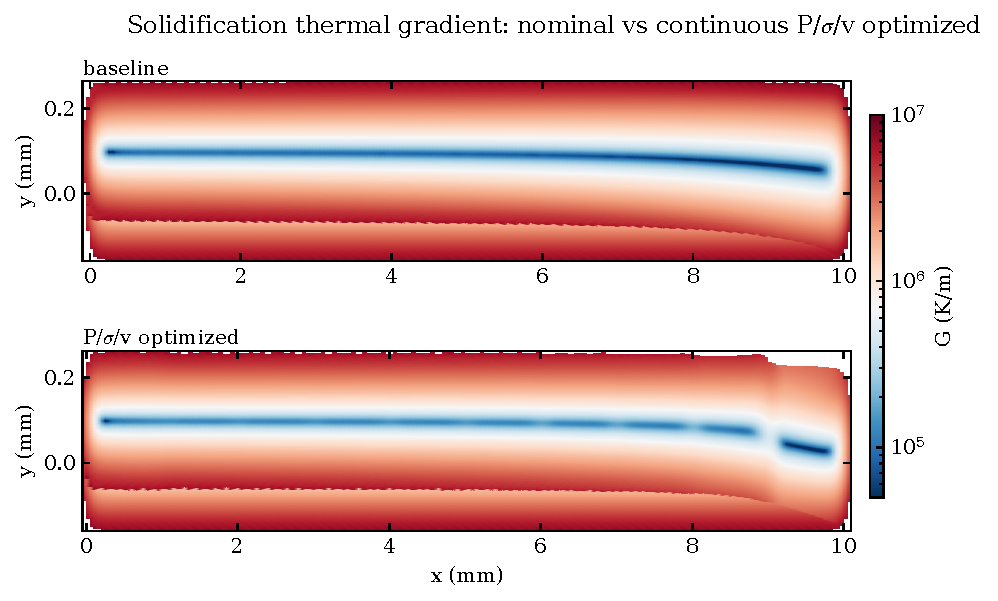
\includegraphics[width=\textwidth]{twotrack_base_maps.pdf}
\caption{Surface solidification thermal-gradient maps for the nominal
serpentine (top) and the $1$~mm continuous $P/\sigma/v$ optimized schedule
(bottom), on a common logarithmic colour scale.}
\label{fig:twotrack-maps}
\end{figure}

\begin{figure}[H]
\centering
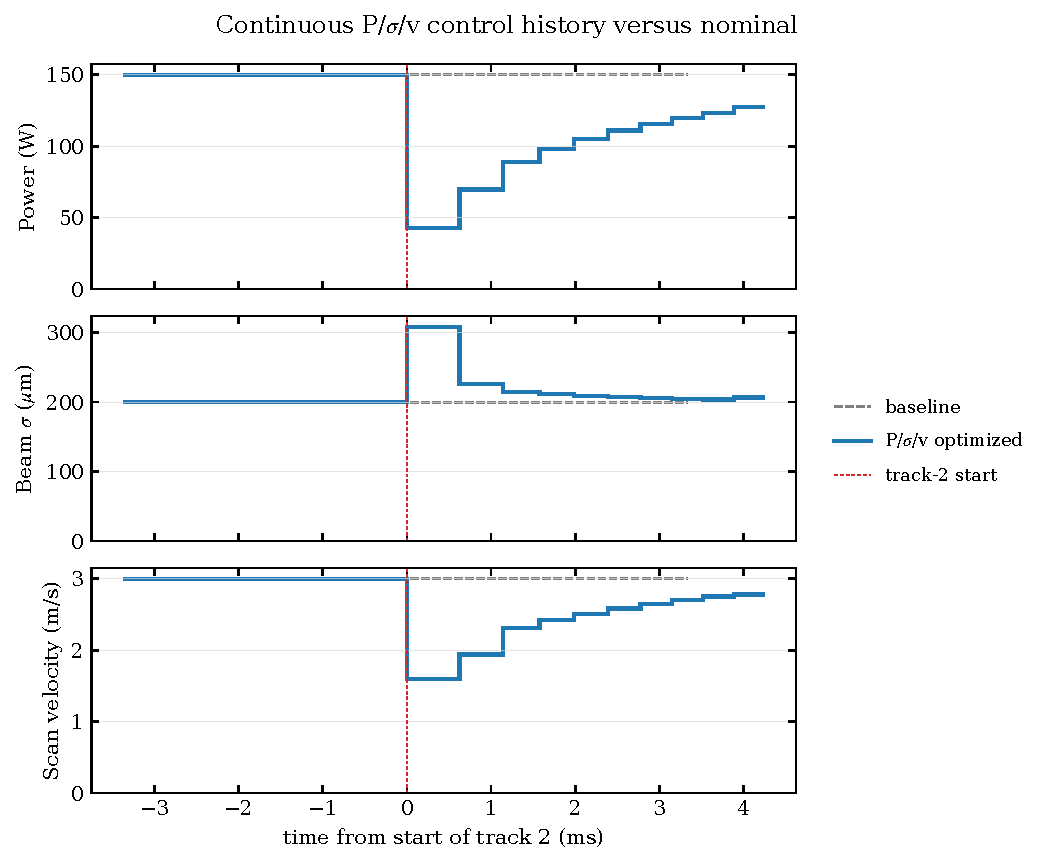
\includegraphics[width=\textwidth]{twotrack_base_controls.pdf}
\caption{Power, lateral beam width, and scan-speed histories for the $1$~mm
continuous schedule against the nominal baseline. The track-2 start is aligned
at zero; the controller slows and cools at the turnaround, then ramps smoothly
back toward nominal.}
\label{fig:twotrack-controls}
\end{figure}

\begin{figure}[H]
\centering
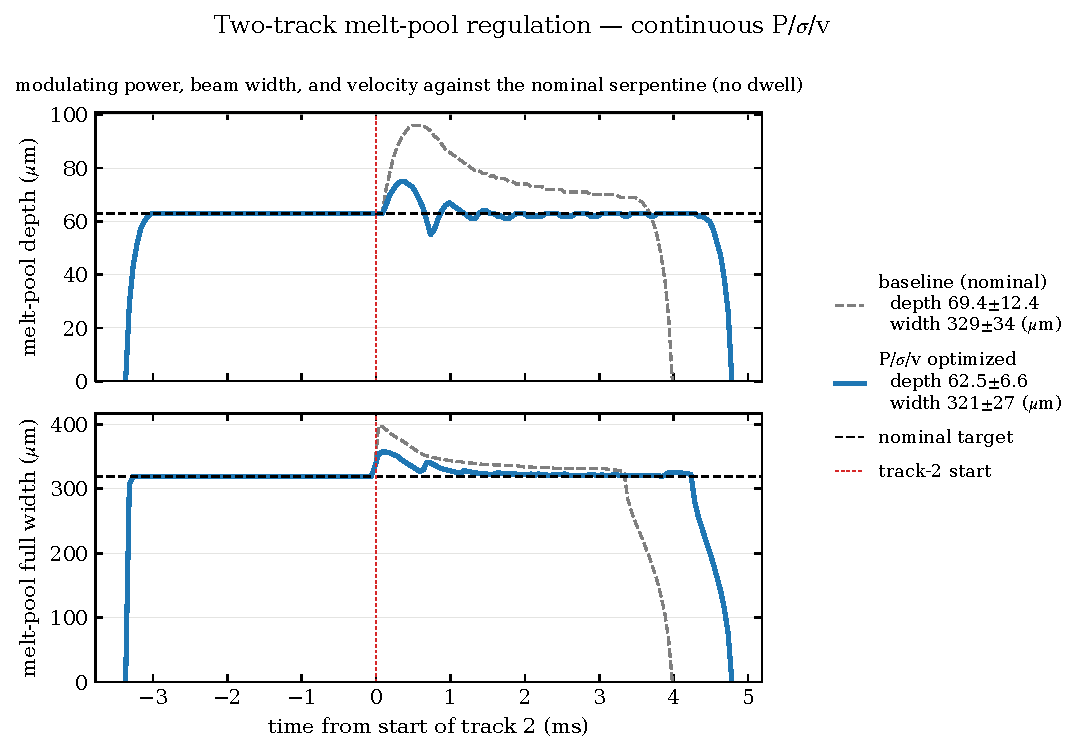
\includegraphics[width=\textwidth]{twotrack_base_traces.pdf}
\caption{Melt-pool depth and full-width traces for the nominal baseline and the
selected $1$~mm continuous $P/\sigma/v$ controller. The baseline overshoots at
the turnaround and decays slowly; the optimized schedule holds the developed
target. The complete block-length sweep is reported in
Table~\ref{tab:twotrack-block}.}
\label{fig:twotrack-traces}
\end{figure}

\subsection{Square raster}
\label{sec:results:square}

The $10\times10$~mm square is the first full raster geometry considered and
consists of 101 equal-length scan tracks. Continuous serpentine scanning is
used throughout, with the power, lateral beam width, and scan velocity
modulated over $1$~mm control blocks. This case tests whether the melt-pool
dimensions can be controlled in a simple raster geometry.

\begin{table}[H]
\centering
\small
\begin{tabular}{lccc}
\toprule
schedule & depth ($\mu$m) & full width ($\mu$m)
& volume (mm$^3$)\\
\midrule
baseline  & $106.0 \pm 12.7$ & $388 \pm 27$ & $0.0798 \pm 0.0240$\\
optimized & $\mathbf{62.2 \pm 2.5}$ & $\mathbf{323 \pm 9.9}$
& $\mathbf{0.01293 \pm 0.00127}$\\
\bottomrule
\end{tabular}
\caption{Square-raster beam-on melt-pool statistics under continuous
serpentine scanning (mean~$\pm$~standard deviation) from full tracked replays
on the $50/10/1~\mu$m grid.}
\label{tab:square-results}
\end{table}

The optimized schedule brings the mean depth and width to the single-track
targets while reducing their variation. The depth standard deviation falls
from $12.7$ to $2.5~\mu$m and the full-width standard deviation falls from
$27$ to $9.9~\mu$m.

\begin{figure}[H]
\centering
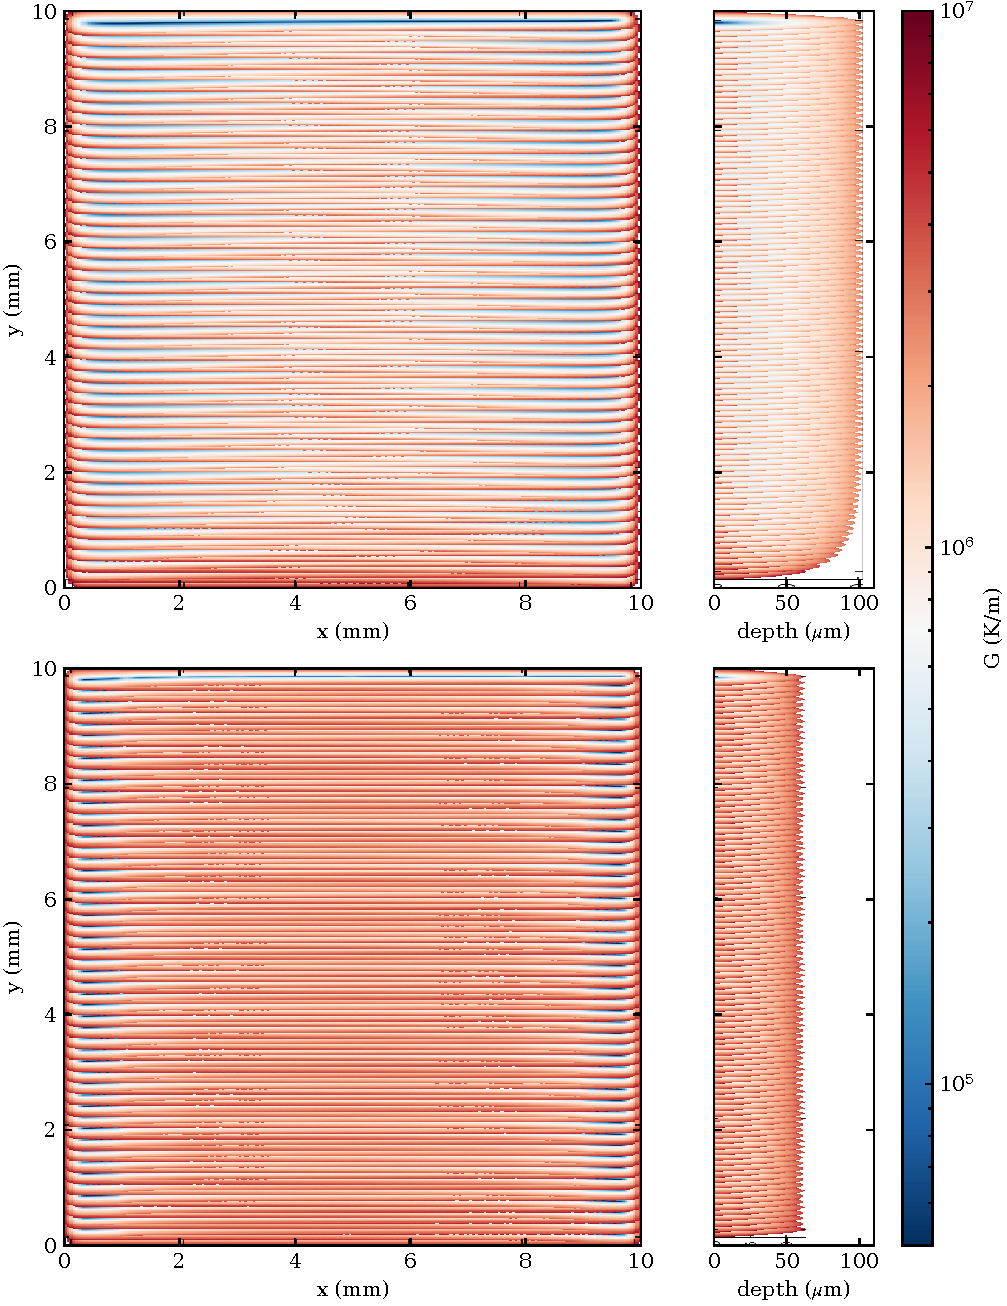
\includegraphics[width=0.88\textwidth]{square_maps_zero.pdf}
\caption{Square-raster solidification thermal-gradient maps under continuous
serpentine scanning. The top-surface map (left) and vertical centre section
(right) are shown for the baseline (top) and $1$~mm optimized (bottom)
schedules.}
\label{fig:square-maps-zero}
\end{figure}

\begin{figure}[H]
\centering
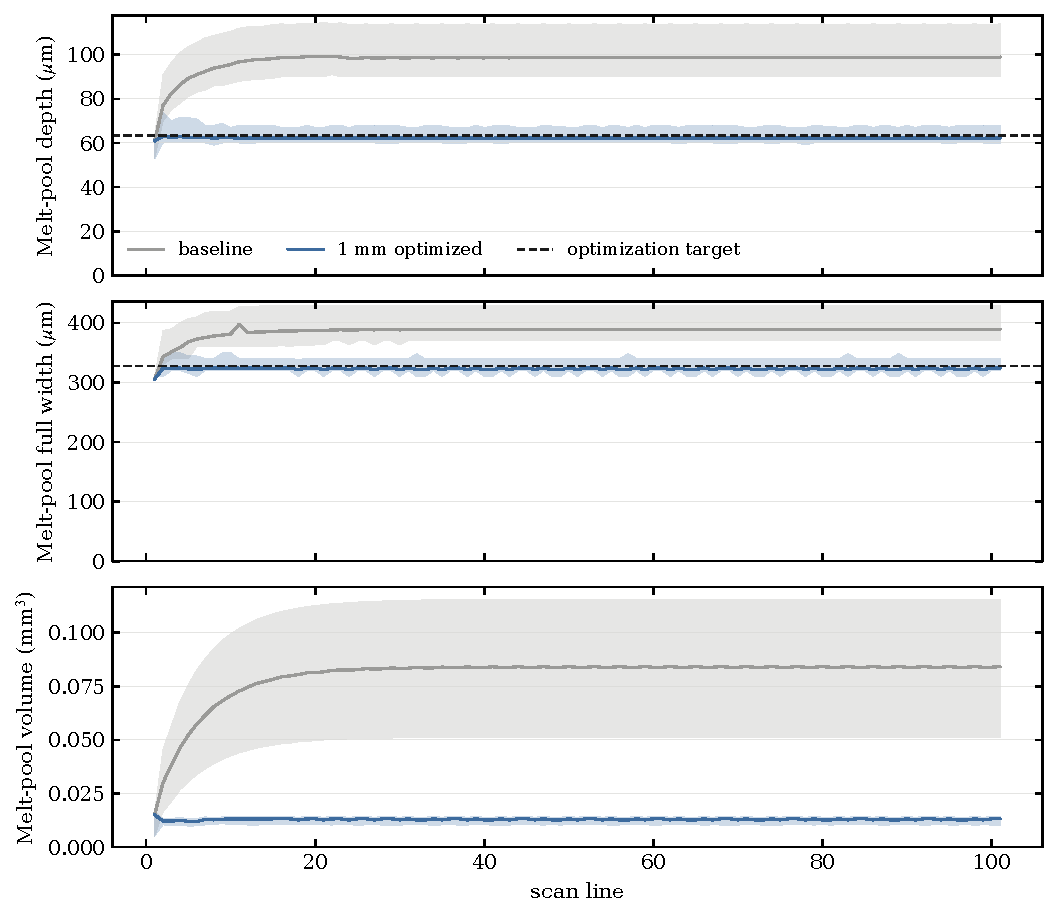
\includegraphics[width=.90\textwidth]{square_traces_zero.pdf}
\caption{Square-raster per-line melt-pool statistics under continuous
serpentine scanning for the baseline and $1$~mm optimized schedules.}
\label{fig:square-traces-zero}
\end{figure}

\begin{figure}[H]
\centering
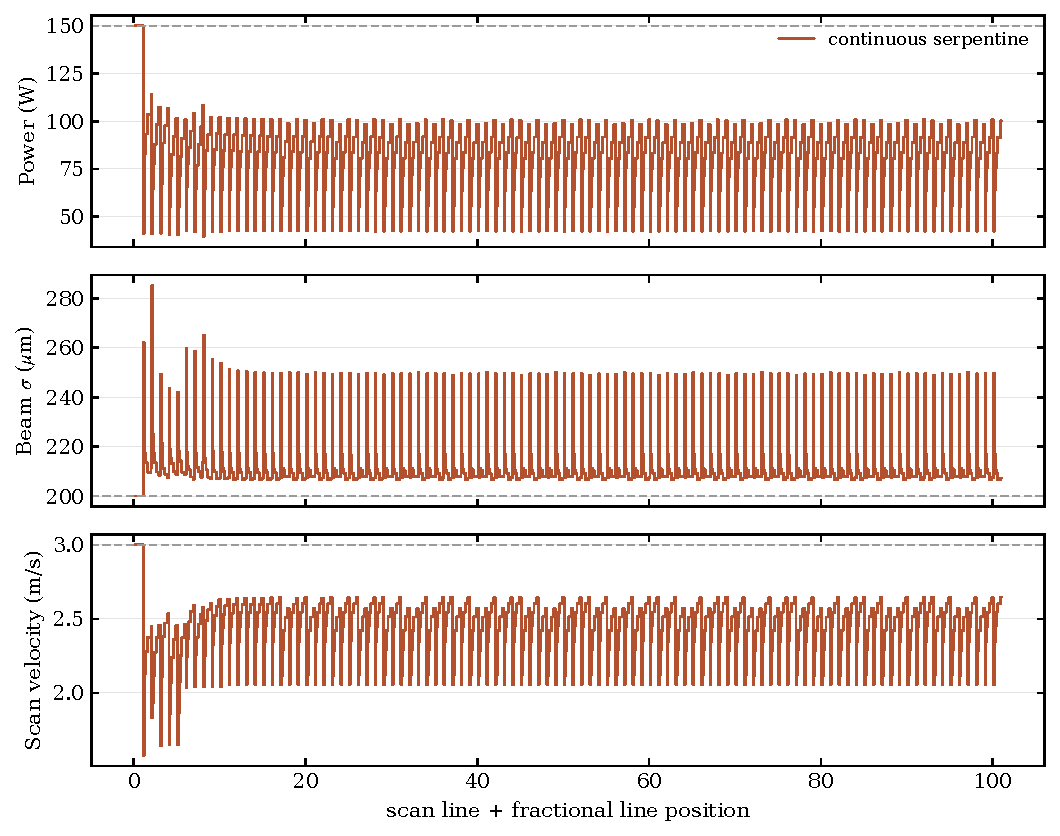
\includegraphics[width=\textwidth]{square_process_parameters.pdf}
\caption{Optimized power, lateral beam width, and scan-speed histories for
the square raster under continuous serpentine scanning.}
\label{fig:square-controls}
\end{figure}

\subsection{Triangle raster}
\label{sec:results:triangle}

The equilateral triangle has $10$~mm sides and consists of 87 scan tracks
whose lengths decrease towards the apex. Continuous serpentine scanning is
used throughout, with the power, lateral beam width, and scan velocity
modulated over nominally $1$~mm control blocks. This case tests whether the
melt-pool dimensions can be controlled as the scan-track length progressively
decreases. The blocks on each track are balanced so that a short remainder is
not left at the end of the track.

\begin{table}[H]
\centering
\small
\begin{tabular}{lccc}
\toprule
schedule & depth ($\mu$m) & full width ($\mu$m)
& volume (mm$^3$)\\
\midrule
baseline  & $118.7 \pm 21.2$ & $484 \pm 170$ & $0.11274 \pm 0.04715$\\
optimized & $\mathbf{63.7 \pm 4.4}$ & $\mathbf{329 \pm 15}$
& $\mathbf{0.01176 \pm 0.00160}$\\
\bottomrule
\end{tabular}
\caption{Triangle-raster beam-on melt-pool statistics under continuous
serpentine scanning (mean~$\pm$~standard deviation) from full tracked replays
on the $50/10/1~\mu$m grid.}
\label{tab:triangle-results}
\end{table}

The optimized schedule brings the mean depth and width to the single-track
targets while reducing their variation. The depth standard deviation falls
from $21.2$ to $4.4~\mu$m and the full-width standard deviation falls from
$170$ to $15~\mu$m.

\begin{figure}[H]
\centering
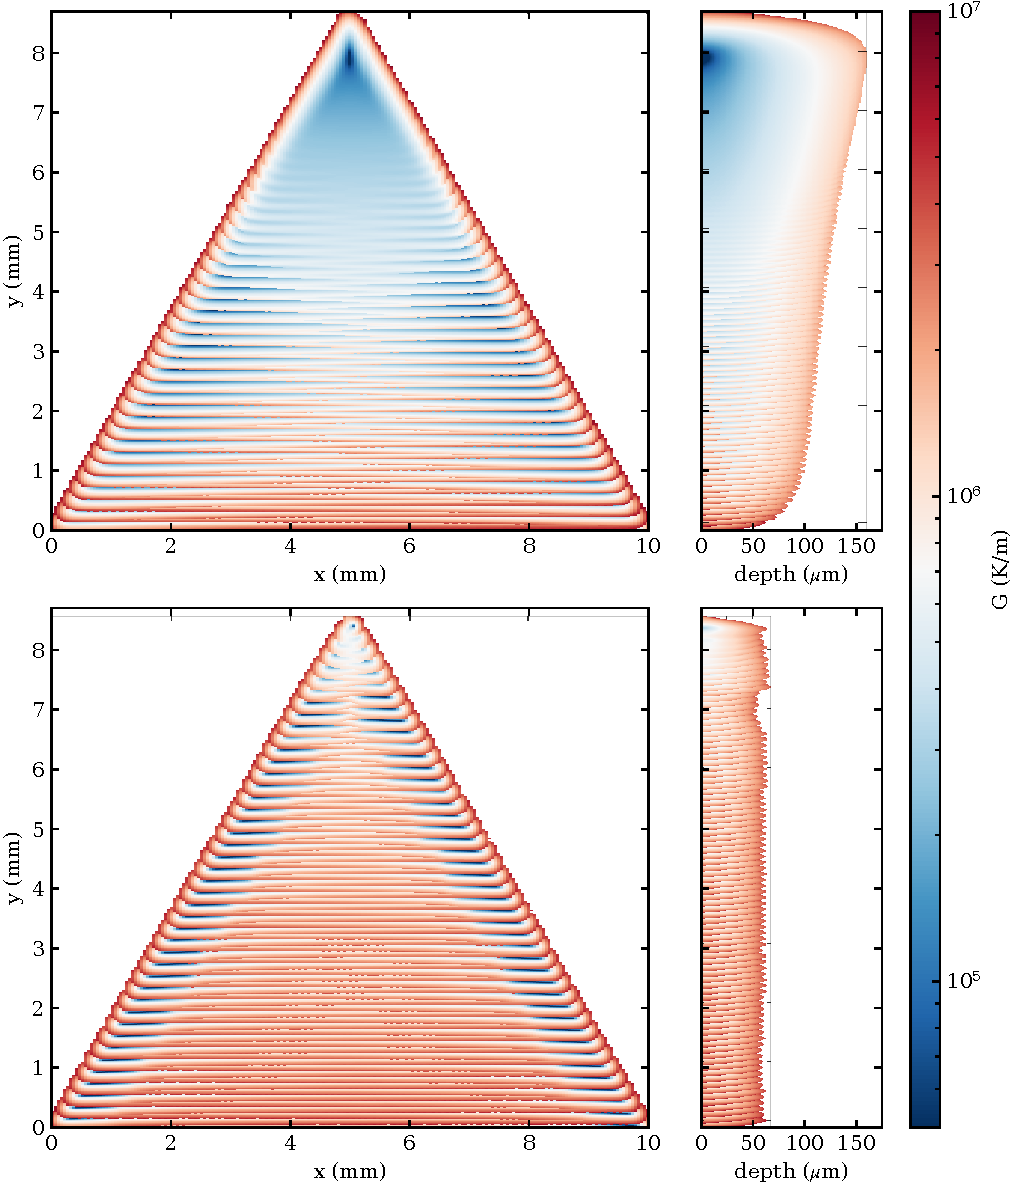
\includegraphics[width=0.88\textwidth]{triangle_maps_zero.pdf}
\caption{Triangle-raster solidification thermal-gradient maps under continuous
serpentine scanning. The top-surface map (left) and vertical centre section
(right) are shown for the baseline (top) and $1$~mm optimized (bottom)
schedules.}
\label{fig:triangle-maps-zero}
\end{figure}

\begin{figure}[H]
\centering
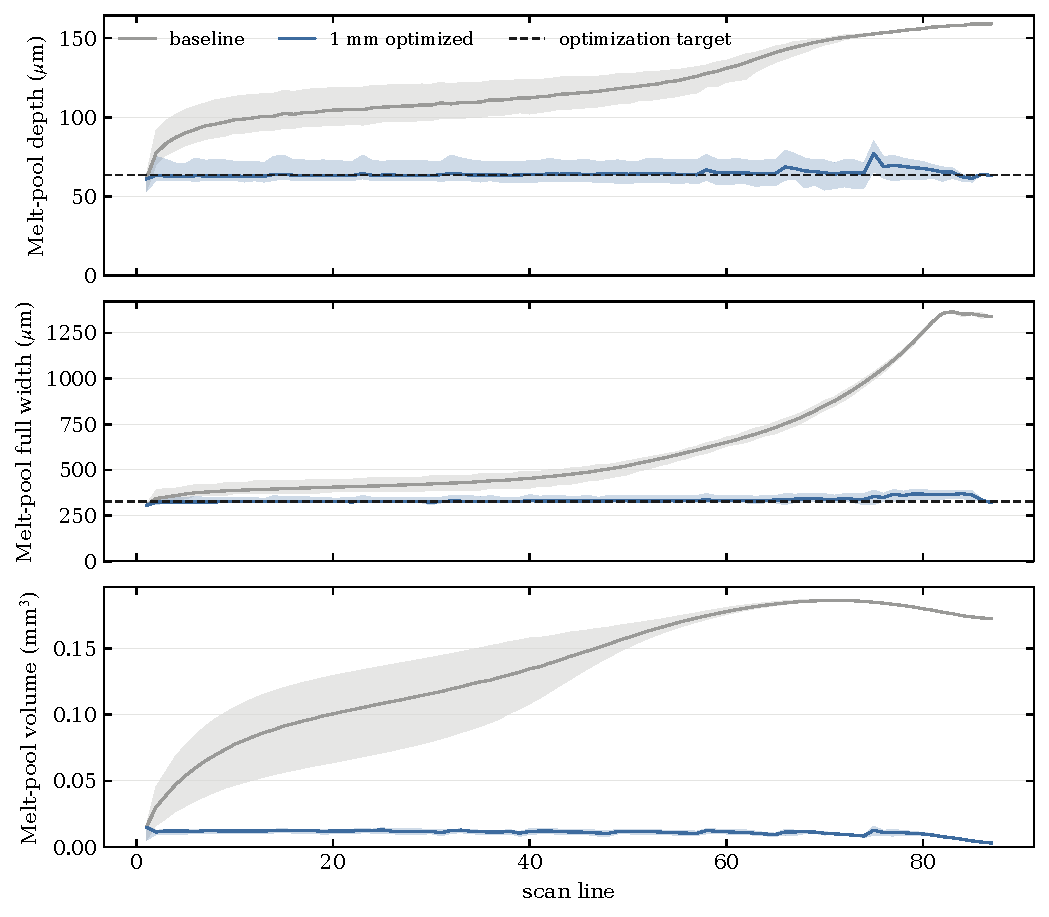
\includegraphics[width=.90\textwidth]{triangle_traces_zero.pdf}
\caption{Triangle-raster per-line melt-pool statistics under continuous
serpentine scanning for the baseline and $1$~mm optimized schedules.}
\label{fig:triangle-traces-zero}
\end{figure}

\begin{figure}[H]
\centering
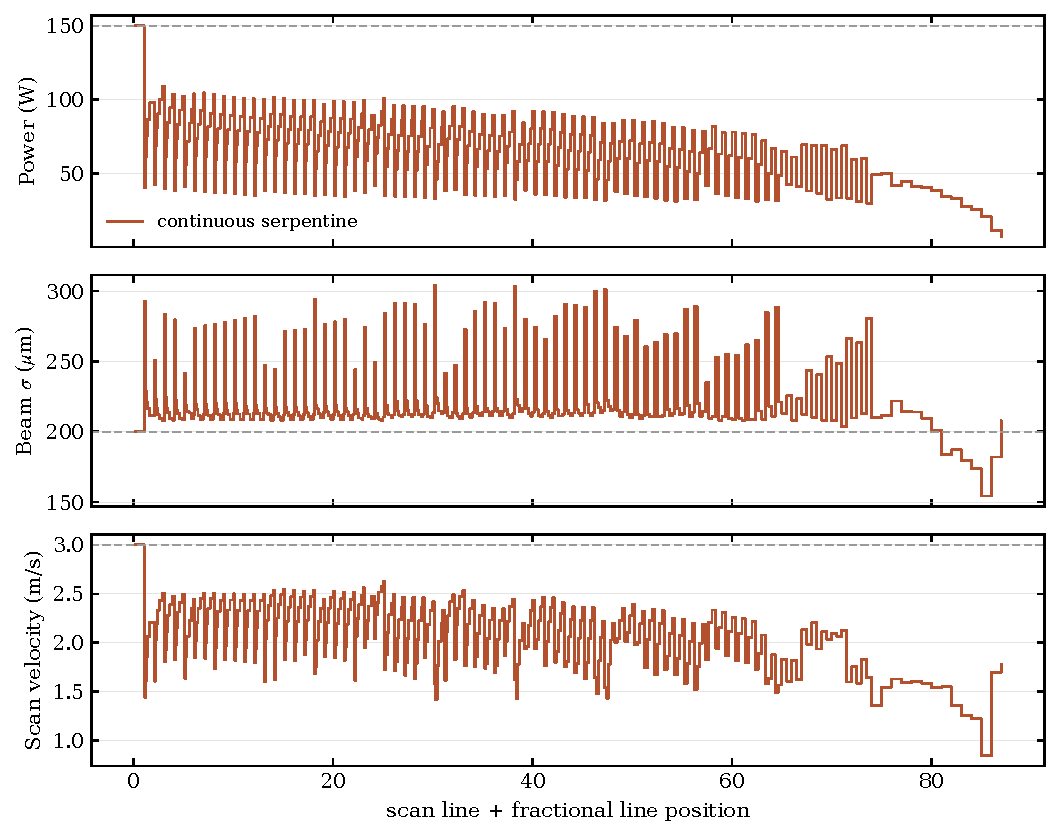
\includegraphics[width=\textwidth]{triangle_process_parameters.pdf}
\caption{Optimized power, lateral beam width, and scan-speed histories for
the triangle raster under continuous serpentine scanning.}
\label{fig:triangle-controls}
\end{figure}

\section{Discussion}
\label{sec:discussion}

The studies above use continuous serpentine scanning and modulate only the
continuous process controls---power, beam width, and scan velocity. A natural
extension is to admit the turnaround dwell as an additional free control, so
that the optimizer sizes a beam-off interval alongside the continuous
parameters. This more elaborate strategy is left to a future study.

\section{Conclusion}
\label{sec:conclusion}

\bibliographystyle{plain}
\bibliography{references}

\end{document}
